
\documentclass[a4paper,12pt]{book}
\usepackage[utf8]{inputenc}
\usepackage[T1]{fontenc}
\usepackage[frenchb]{babel} 
\usepackage{a4wide}
\usepackage{graphicx}
\graphicspath{{images/}}
\usepackage{subfig}
\usepackage{tikz}
\usetikzlibrary{shapes,arrows}
\usepackage{pgfplots}
\pgfplotsset{compat=newest}
\pgfplotsset{plot coordinates/math parser=false}
\newlength\figureheight
\newlength\figurewidth
\pgfkeys{/pgf/number format/.cd,
set decimal separator={,\!},
1000 sep={\,},
}
\usepackage{ifthen}
\usepackage{ifpdf}
\ifpdf
\usepackage[pdftex]{hyperref}
\else
\usepackage{hyperref}
\fi
\usepackage{color}
\hypersetup{%
colorlinks=true,
linkcolor=black,
citecolor=black,
urlcolor=black}

\renewcommand{\baselinestretch}{1.05}
\usepackage{fancyhdr}
\pagestyle{fancy}
\fancyfoot{}
\fancyhead[LE,RO]{\bfseries\thepage}
\fancyhead[RE]{\bfseries\nouppercase{\leftmark}}
\fancyhead[LO]{\bfseries\nouppercase{\rightmark}}
\setlength{\headheight}{15pt}

\let\headruleORIG\headrule
\renewcommand{\headrule}{\color{black} \headruleORIG}
\renewcommand{\headrulewidth}{1.0pt}
\usepackage{colortbl}
\arrayrulecolor{black}

\fancypagestyle{plain}{
  \fancyhead{}
  \fancyfoot[C]{\thepage}
  \renewcommand{\headrulewidth}{0pt}
}

\makeatletter
\def\@textbottom{\vskip \z@ \@plus 1pt}
\let\@texttop\relax
\makeatother

\makeatletter
\def\cleardoublepage{\clearpage\if@twoside \ifodd\c@page\else%
  \hbox{}%
  \thispagestyle{empty}%
  \newpage%
  \if@twocolumn\hbox{}\newpage\fi\fi\fi}
\makeatother

\usepackage{amsthm}
\usepackage{amssymb,amsmath,bbm}
\usepackage{array}
\usepackage{bm}
\usepackage{multirow}
\usepackage[footnote]{acronym}

\newcommand*{\SET}[1]  {\ensuremath{\mathbf{#1}}}
\newcommand*{\VEC}[1]  {\ensuremath{\boldsymbol{#1}}}
\newcommand*{\FAM}[1]  {\ensuremath{\boldsymbol{#1}}}
\newcommand*{\MAT}[1]  {\ensuremath{\boldsymbol{#1}}}
\newcommand*{\OP}[1]  {\ensuremath{\mathrm{#1}}}
\newcommand*{\NORM}[1]  {\ensuremath{\left\|#1\right\|}}
\newcommand*{\DPR}[2]  {\ensuremath{\left \langle #1,#2 \right \rangle}}
\newcommand*{\calbf}[1]  {\ensuremath{\boldsymbol{\mathcal{#1}}}}
\newcommand*{\shift}[1]  {\ensuremath{\boldsymbol{#1}}}

\newcommand{\eqdef}{\stackrel{\mathrm{def}}{=}}
\newcommand{\argmax}{\operatornamewithlimits{argmax}}
\newcommand{\argmin}{\operatornamewithlimits{argmin}}
\newcommand{\ud}{\, \mathrm{d}}
\newcommand{\vect}{\text{Vect}}
\newcommand{\sinc}{\ensuremath{\mathrm{sinc}}}
\newcommand{\esp}{\ensuremath{\mathbb{E}}}
\newcommand{\hilbert}{\ensuremath{\mathcal{H}}}
\newcommand{\fourier}{\ensuremath{\mathcal{F}}}
\newcommand{\sgn}{\text{sgn}}
\newcommand{\intTT}{\int_{-T}^{T}}
\newcommand{\intT}{\int_{-\frac{T}{2}}^{\frac{T}{2}}}
\newcommand{\intinf}{\int_{-\infty}^{+\infty}}
\newcommand{\Sh}{\ensuremath{\boldsymbol{S}}}
\newcommand{\C}{\SET{C}}
\newcommand{\R}{\SET{R}}
\newcommand{\Z}{\SET{Z}}
\newcommand{\N}{\SET{N}}
\newcommand{\K}{\SET{K}}
\newcommand{\reel}{\mathcal{R}}
\newcommand{\imag}{\mathcal{I}}
\newcommand{\cmnr}{c_{m,n}^\reel}
\newcommand{\cmni}{c_{m,n}^\imag}
\newcommand{\cnr}{c_{n}^\reel}
\newcommand{\cni}{c_{n}^\imag}
\newcommand{\tproto}{g}
\newcommand{\rproto}{\check{g}}
\newcommand{\LR}{\mathcal{L}_2(\SET{R})}
\newcommand{\LZ}{\ell_2(\SET{Z})}
\newcommand{\LZI}[1]{\ell_2(\SET{#1})}
\newcommand{\LZZ}{\ell_2(\SET{Z}^2)}
\newcommand{\diag}{\operatorname{diag}}
\newcommand{\noise}{z}
\newcommand{\Noise}{Z}
\newcommand{\filtnoise}{\zeta}
\newcommand{\tp}{g}
\newcommand{\rp}{\check{g}}
\newcommand{\TP}{G}
\newcommand{\RP}{\check{G}}
\newcommand{\dmin}{d_{\mathrm{min}}}
\newcommand{\Dmin}{D_{\mathrm{min}}}
\newcommand{\Image}{\ensuremath{\text{Im}}}
\newcommand{\Span}{\ensuremath{\text{Span}}}

\newtheoremstyle{break}
  {11pt}{11pt}%
  {\itshape}{}%
  {\bfseries}{}%
  {\newline}{}%
\theoremstyle{break}

%\theoremstyle{definition}
\newtheorem{definition}{Définition}[chapter]

%\theoremstyle{definition}
\newtheorem{theoreme}{Théorème}[chapter]

%\theoremstyle{remark}
\newtheorem{remarque}{Remarque}[chapter]

%\theoremstyle{plain}
\newtheorem{propriete}{Propriété}[chapter]
\newtheorem{exemple}{Exemple}[chapter]

\parskip=5pt
%\sloppy

\begin{document}

%%%%%%%%%%%%%%%%%%
%%% First page %%%
%%%%%%%%%%%%%%%%%%

\begin{titlepage}
\begin{center}


\includegraphics[width=0.6\textwidth]{uvsq-logo-rvb-def}\\[1cm]

{\large Sécurité des Contenus, des Réseaux, des Télécommunications et des Systèmes}\\[0.5cm]

{\large Rapport de stage}\\[0.5cm]

% Title
\rule{\linewidth}{0.5mm} \\[0.4cm]
{ \huge \bfseries Amélioration des process d'audit et de collecte des indicateurs de sécurité des sites web publics du groupe Schneider-Electric\\[0.4cm] }
Société d'accueil : Schneider-Electric Grenoble
\rule{\linewidth}{0.5mm} \\[1.5cm]


% Author and supervisor
\noindent
\begin{minipage}{0.4\textwidth}
  \begin{flushleft} \large
    \emph{Auteur :}\\
    M. Pazisnéwendé Aubain  \textsc{Tapsoba}\\

  \end{flushleft}
\end{minipage}%
\begin{minipage}{0.4\textwidth}
  \begin{flushright} \large
    \emph{Maître de stage :} \\
    Mme. Siham \textsc{Benhamidouche}\\
  
  \end{flushright}
\end{minipage}

\vfill

% Bottom of the page
{\large Période du 03 Avril au 03 Octobre \\ Année académique 2017-2018}

\end{center}
\end{titlepage}

%%%%%%%%%%%%%%%%%%%%%%%%%%%%%
%%% Non-significant pages %%%
%%%%%%%%%%%%%%%%%%%%%%%%%%%%%

\frontmatter
\chapter*{Dédicaces}
Nous dédions ce document à notre famille.
\chapter*{Remerciements}
Par ces lignes nous exprimons nos sincères remerciements, d’abord à l’endroit de toute l’équipe pédagogique de l'Université de Versailles Saint-Quentin-En-Yvelines pour notre formation.


Nous remercions ensuite Schneider-Electric de nous avoir ouvert ses portes pour notre stage.
Plus particulièrement, nos remerciements sincères aux personnes suivantes :
\begin{itemize}
    \item Siham Benhamidouche, notre maître de stage;
    \item Lionel Triay et Maurizio Molina pour leur encadrement et leur bienveillance tout au long de notre stage;
    \item Jerome Covini, Jerome Bourgeon et Emmanuel Beaugrand pour leurs participations sincères dans nos projets et leurs conseils.
\end{itemize} 

Enfin nous témoignons notre gratitude à tous ceux qui n’ont ménagé aucun effort pour l’aboutissement de notre formation. 

\clearpage
\tableofcontents

\clearpage
\listoffigures

\clearpage
\chapter*{Liste des sigles et acronymes}
\begin{acronym}[CP-OFDMX] % Give the longest acronym here
\acro{DEVOPS}{\emph{Developement and Operations}}
\acro{FBI}{\emph{Federal Business Intelligence}}
\acro{DEVSECOPS}{\emph{Development Security Operations}}
\acro{POC}{\emph{Proof Of Concept}}
\acro{OWASP}{\emph{Open Web Application Security Project}}
\acro{FQDN}{\emph{Full Qualified Domain Name}}
\acro{CNs}{\emph{Common Name}}
\acro{SANs}{\emph{Server Alternative Name}}
\acro{HTTP}{\emph{HyperText Transfert Protocol}}
\acro{SDLC}{\emph{Software Development Life Cycle}}
\acro{SCRUM}{\emph{test}}
\end{acronym}

%%%%%%%%%%%%%%%%%%%%%%%%%%%%%%%%%%%%%%%%%%%%
%%% Content of the report and references %%%
%%%%%%%%%%%%%%%%%%%%%%%%%%%%%%%%%%%%%%%%%%%%

\mainmatter
\pagestyle{fancy}

\cleardoublepage

\chapter*{Introduction générale}
\vspace*{-1.1cm}
Les thématiques de la sécurité informatique s’invitent depuis plusieurs années au sujet des préoccupations majeures des organisations et des entreprises. 
De son ampleur, certaines entreprises à juste titre lui confèrent le titre de domaine critique et sensible. 
Selon les conclusions du rapport de Verizon parut en 2017, 77\% des organisations dans le monde ont été touchées par des cyber-attaques au cours de l’année 2017. \newline
Ces attaques ont des impacts forts sur l’économie et sur la réputation des victimes. Dans ce contexte, il apparaît clairement la nécessité pour les entreprises d’améliorer la sécurité de leur système d’information.
Ce processus d’amélioration passe par la formation de la ressource humaine d’une part et par des réalisations techniques sûres d’autre part. \newline
En particulier, techniquement, l’amélioration de la sécurité d’une entreprise se produit en amont de la phase de production par l’amélioration de la sécurité et en aval par la mise en place de techniques de défense, de détection et de gestion des incidents de sécurité.\newline
La maîtrise de ces techniques est la problématique actuelle des acteurs de la cybersécurité et de toutes les entreprises émettant des produits électroniques et informatiques. \\
Ainsi afin de s’assurer la maîtrise de ces processus, Schneider-Electric s'est doté de plusieurs pôles dédiés au monitoring, à la gestion des incidents et à la prévention de ces derniers. 

De ces besoins exprimés, nous avons été accueillis au sein du groupe Schneider-Electric pour un stage de six mois (06) mois durant lequel, nous avons travaillé sur l’amélioration des indicateurs de sécurité de notre société d'accueil d'une part et sur la mise en place d'un \ac{POC} de certification continue d'autre part. 
\newline Notre stage au sein du groupe Schneider-Electric s’est construit autour du sujet « Amélioration des indicateurs de sécurité des sites web publics du groupe Schneider-Electric », nous avons de ce fait travaillé sur l’intégration des indicateurs de sécurité en amont de la phase de production et en avale sur le monitoring des indicateurs de sécurité. 
\newline Le présent document, synthèse de nos activités durant le stage s’articule sur trois (03) parties. \\
Dans la première partie, nous procéderons à la présentation de notre entreprise d’accueil, ainsi que les objectifs généraux de notre stage. 
\newline
Dans la deuxième partie, nous présenterons d'abord les métiers que nous avons appris, ensuite nous aborderons nos propositions pour l'amélioration de ces métiers.
\newline
Dans la troisième partie du rapport, il sera question de nos réalisations dans la mise en  œuvre d'un POC pour la mise en  œuvre des concepts de certification continue dans le cadre d'un projet \ac{DEVOPS}.

\part{Etudes préalables }
\chapter{La société d'accueil}
\section*{Introduction}
L'objet de ce chapitre est de présenter la société d'accueil. Pour cela il sera procédé dans ce chapitre à la présentation de Schneider-Electric, cela dans le but de mieux appréhender les enjeux de notre stage. 

\section{Présentation}
Schneider-Electric est une multinationale Française spécialisée dans les automatismes et dans la gestion de l’énergie.\newline 
Elle intervient particulièrement dans la conception, la gestion, la réalisation des solutions techniques innovantes et dans la proposition de services autour des projets électriques. \newline
Sa mission principale est de mettre à la disposition de ses clients des produits à haute valeur ajoutée afin de les accompagner dans leur stratégie de gestion de l’énergie.\newline


Fondée au 19è siècle par les frères Schneider, la société a en 180 années su relever de nombreux défis et devenir un acteur majeur à tous les niveaux des offres électriques. De nos jours, elle se positionne comme une entreprise innovante, et engagée dans la transition énergétique, dans le développement des outils intelligents et dans la formation des jeunes.


Sur le territoire Français la société compte plus de 100 sites, plus de 150 milles collaborateurs et produit un chiffre d'affaire annuel supérieur à 1,7 milliard d'euros depuis 2013.\newline
De son leadership dans son domaine, elle est la cible de plusieurs attaques informatiques. Ces attaques visent pour l’essentiel la base de connaissance du groupe, et pour d’autres l'objectif est de ternir la réputation de la société auprès de ses clients.
Aussi il importe de mettre aux devants, vu l'importance du groupe, les potentiels espionnages dont il pourrait être l'objet.


\section{Organisation interne}
Schneider-Electric est une société européenne à conseil d’administration. Elle applique le code de gouvernance des entreprises et des sociétés cotées. 
Selon les recommandations de cette gouvernance, elle dispose d’un conseil d’administration en charge de déterminer les orientations de l’activité de la société et veille à leur mise en œuvre. 
\newline 
A la suite du conseil d'administration suivent respectivement la direction du groupe et le comité exécutif. La direction du groupe représente la société dans ses rapports avec les tiers. Elle est investie des pouvoirs les plus étendus pour agir en toutes circonstances au nom de la société. 
\newline
Le comité exécutif, quant à lui est en charge de supporter et de mettre en opération les décisions du conseil d'administration. 

\section{Aperçu sur l'architecture Informatique}
De par son choix de développement et de sa répartition géographique, la société dispose d’une architecture informatique distribuée et hétérogène.
De partout dans le monde, elle dispose de plusieurs datacenters sur lesquels sont déployés les applications dites sensibles.
\newline
A côté de ces applications dites sensibles, il en existe celles à faible valeur ajoutée qui se retrouvent souvent chez des fournisseurs tiers.

Aussi certaines acquisitions du groupe gère elle-même leur système d’information qui n’ont souvent aucune connexion avec celui du groupe. Cette situation singulière intervient particulièrement lorsque l'intégration du système d'information de la société rachetée va entraîner une régression de sécurité chez l'une des deux sociétés. 

\section{Quelques attaques informatiques sur le groupe}
Faisant un stage en sécurité informatique au sein du groupe, il nous a paru nécessaire de recenser les attaques et les vulnérabilités marquantes auxquelles le groupe a déjà été exposé.  
\subsection{Exploitation d'une vulnérabilité sur le triconnex}
Cette attaque fut signalée par la \ac{FBI}. Elle date de l’année 2015. Elle a touché une filiale du groupe spécialisée dans le développement des logiciels de supervision de pipeline. Cette attaque a eu pour conséquence l’exfiltration de données massives. 
\newline
Par ailleurs, elle a eu des conséquences économiques, et a également eu des impacts négatifs sur la réputation du groupe.  

\subsection{Vulnérabilités sur le SCADA}
De façon chronologique, il eût d'abord celles de Septembre 2012. En effet, durant cette période, la filiale TELVENT de Schneider-Electric, spécialisée dans les systèmes de contrôles industriels énergétiques, a été victime d’une attaque réseau. Des attaquants d’origine chinoise ont réussi à contourner les pares-feux de TELVENT, et, après avoir investi des pans entiers de son réseau, y ont installé des logiciels malicieux afin de dérober des données sur un \ac{SCADA}.
\newline
Ensuite, en 2018, de multiples vulnérabilités ont été découvertes dans SCADA les produits Schneider-Electric le 12 février 2018 par le \ac{CERT} de la France. Elles permettent à un attaquant de provoquer une exécution de code arbitraire à distance, une atteinte à l'intégrité des données et une atteinte à la confidentialité des données.

\section*{Conclusion}
Dans ce chapitre, nous avons eu un aperçu général sur les domaines d'intervention du groupe d'une part et d'autre part sur son organisation interne. 
\\Ce chapitre nous a permis de nous familiariser avec la société et de mieux connaître ses domaines d'activités. Aussi il nous a permis de mieux comprendre les enjeux de la sécurité informatique pour la société d'accueil. 

\chapter{Contexte du stage}
\section*{Introduction}
Dans ce chapitre, nous présenterons d'abord les objectifs assignés à notre stage et les attentes de l'entreprise d'accueil, ensuite les compléments souhaités de ce stage à notre formation pédagogique.

\section{Le stage}
Le Master II SeCReTS est une formation de l’université Paris-Saclay, un consortium de trois universités, de neuf grandes écoles et de sept organismes de recherches. \newline
Cette formation a pour but d’apporter aux étudiants une compréhension fine des défis liés d’une part, à la conception des systèmes sûrs et d’autres part à fournir des bases théoriques, pratiques et solides sur les concepts et les enjeux de la cybersécurité. \newline
La validation de ce Master est jalonnée par un stage de six mois et obligatoire à réaliser auprès des professionnels de la sécurité informatique. 
En particulier, ce stage a pour objectifs : 
\begin{itemize}
    \item[•]	de nous permettre d’apprendre de notre futur métier ;
    \item [•]	de nous donner un encadrement avant notre immersion totale dans le monde professionnel ;
    \item [•]	de permettre à l'école de profiter des retours des entreprises afin de mieux adapter la formation. 
\end{itemize}


Dans le cadre de ma formation, j’ai été reçu en stage de six (06) mois au sein de l’équipe DCX Security de la société Schneider-Electric. Dans cette équipe nous avons pu travailler principalement sur le sujet \textbf{« Amélioration des process d'audit et de collecte des indicateurs de sécurité des sites web publics du groupe Schneider-Electric »}. 

Ce stage devrait être l’occasion pour nous d’approfondir nos connaissances sur les sujets de la sécurité des applications web en particulier, dans la sécurité opérationnelle, dans le monitoring et dans la réponse aux incidents des applications web en général. 

\section{Equipe d’accueil}
\subsection{Présentation}
Nous avons été accueillis au sein de l’équipe DCX Security. Cette équipe est managée par Siham Benhamidouche, Digital Risk Leader, et compte en tout trois (03) collaborateurs.


Elle est entre autres en charge de la sécurité des applications web, de celle du \ac{DNS} et de celle des applications sensibles. 
\newline Particulièrement les objectifs principaux de l’équipe sont de veiller à la sécurité des applications web et mobiles publiques du groupe, ceci, en passant par la surveillance des indicateurs de sécurité des sites web publics.


Pour l’atteinte de ses objectifs, elle passe par plusieurs missions telles que des séances formation, des campagnes de blocage d'adresses IP et des missions de gestion d'incidents. 
De la rédaction de supports, à l’amélioration des notes, en passant par la gestion des incidents et l’amélioration des process, nous avons pu apporter notre contribution à la vie de l’équipe et à l’atteinte des objectifs assignés à l’équipe. 


\subsection{Objectifs de l'équipe}
A notre arrivée au sein de l'équipe nous avons d’abord voulu comprendre ses métiers. Passée cette étape, nous avons voulu comprendre les difficultés auxquelles faisaient face l’équipe. De cette étape, nous avons pu rassembler les missions suivantes : 
\begin{itemize}
    \item[•] Améliorer les notes de sécurité du groupe Schneider-Electric ; 
    \item[•] Rédiger des politiques et standards de sécurité pour les sites web ;
    \item[•] Rédiger des guides de configurations sûres ;
    \item[•] Sensibiliser sur la sécurité des applications web ; 
    \item[•] Etre le réfèrent technique pour les vulnérabilités web et mobiles; 
    \item[•] Réagir aux incidents de sécurité relatifs aux technologies inhérentes à celles du web.
\end{itemize}
Dans la mise en  œuvre de ses missions, l'équipe fait face à plusieurs difficultés. Parmi ces dernières, nous avons pu observer :
\begin{itemize}
   \item[•] L'identification des propriétaires des systèmes présentant des incidents ;
   \item[•] La distribution du système d’information du groupe ; 
   \item[•] L'anticipation dans l’identification des systèmes présentant des problèmes de sécurité ;
   \item[•] La mise à jour rapide des politiques de sécurité.
\end{itemize}

\section{Objectifs du stage}
Les objectifs de notre stage ont été à la fois de participer à l’atteinte des objectifs de l’équipe et de proposer des solutions aux difficultés exprimées plus haut. En accord avec le sujet du stage « Amélioration des indicateurs de sécurité des sites web publics du groupe SE » nous avons travaillé sur l’amélioration des notes de sécurité du groupe Schneider-Electric en aval et sur la certification des applications en amont. 
Ces travaux devraient permettre à l’équipe de façon générale de : 
\begin{itemize}
    \item[•] améliorer les scores de sécurité du groupe ;
    \item[•] disposer de plus d’outils de checks de la sécurité des applications web ;
    \item[•] intégrer des tests de sécurité durant le processus de certification des applications ;
\end{itemize}

\section{Résultats attendus}
Le résultat général attendu à l'issue de ce stage était l'amélioration des notes de sécurité de Schneider-Electric délivrées par les agences de notation cyber.\newline
Ainsi, étions-nous libre de proposer toute solution qui permettrait d'atteindre ces résultats. 
De par l'orientation de notre formation, nous avons pris position sur les questions techniques. 


Comme résultats particuliers de notre stage, nous devrions proposer des POC  qui aideraient l'équipe à devenir plus efficace d'une part et d'autre part des POC qui permettraient de produire des applications plus sûres et plus conformes aux politiques de sécurité du groupe.

\section*{Conclusion}
Ce chapitre nous a permis de mieux comprendre les missions de notre équipe et de ce fait, d'avoir une meilleure approche pour la réussite de notre stage. A ce sujet il nous a permis d'avoir un aperçu général sur les besoins de l'équipe d'accueil en particulier et sur ceux de la société en générale. 


\part{Amélioration des notes de sécurité du groupe}

\chapter{Etude de l'existant}
\section*{Introduction}
L’objet de ce chapitre est de présenter le système de surveillance de sécurité adopté par le groupe Schneider-Electric. Aussi il aura pour objet de présenter la problématique et les objectifs assignés à cette partie du stage.  

\section{Surveillance de sécurité}
Au vu de son modèle de développement, le groupe a opté pour un système de surveillance géré par des entreprises externes. Ces entreprises sont des agences de notation spécialisées dans la cybersécurité. Elles scannent de façon régulière le réseau Internet et établissent sur la base des remontées des notes qu’elles assignent à ses clients scannés. 


Ce choix se justifie amplement par le besoin pour la société de pouvoir évaluer rapidement et simplement son niveau de cybersécurité. Il s’agit là, d’une attente de la direction générale, toujours dans la volonté de s'auto-évaluer par rapport aux autres entreprises du même secteur, voir à leurs concurrents. 

\section{Les agences de notation cyber}
\subsection{Présentation}
Les agences de notation cyber sont des agences qui attribuent des notes aux entreprises suivant des indicateurs de sécurité visibles et atteignables depuis le réseau internet. 
Ces notes sont visibles à toute personne moyennant un contrat et ont plusieurs finalités. Elles sont d'abord utilisées par les assurances afin de tenir compte des risques cyber, ensuite, elles ont un impact significatif sur la valeur marchande de l'entreprise scannée;  enfin, elles permettent de mieux choisir ses partenaires et d'avoir des indicateurs sur leur maturité en matière de sécurité informatique. 


\subsection{Mode opératoire}
Les plateformes de notation spécialisées en cybersécurité collectent, grâce à différentes sondes et connecteurs sur le réseau Internet, trois types de données :
\begin{itemize}
    \item des données sur les activités malicieuses ; 
    \item des flux de données fournis par les vendeurs, éditeurs de logiciels et de systèmes de sécurité et acteurs spécialisés en threat intelligence ; 
    \item des flux de données propriétaires constitués à partir des analyses de vulnérabilités externes régulières sur les réseaux des entreprises évaluées et des capteurs positionnés en divers endroits du réseau Internet.
\end{itemize}
Ces données sont ensuite agrégées et permettent, grâce à des algorithmes non révélés, d’établir des notes par grands indicateurs, puis une note globale pour chaque société. 
\subsection{Techniques de collectes}
Les techniques de collecte sont fortement dépendantes de l'agence de notation et du type de données à collecter. Nous avons pu observer trois techniques de collectes utilisées par la majorité des agences de notation cyber. 

Les techniques utilisées pour la détection des systèmes éventuellement compromis sont celles du sinkhole et/ou du honeypot. Dans un premier temps,  ces techniques ont pour principe général de diriger tous les flux entrants et sortants de la machine suspecte vers un système sain et contrôlé. Elles permettent également de simuler un comportement normal de la machine compromise. Ensuite, au sein du système contrôlé, elles permettent de scinder les flux normaux des flux malicieux, cela dans l'objectif de faire une analyse de ceux malicieux afin de déterminer le type d’infection dont est l'objet la machine.


Les techniques utilisées pour la détection des spams indésirables sont celles dites de spam trapping. Cette technique permet de simuler une adresse mail qui n’est utilisée par personne, ainsi tous les mails à destination de cette adresse sont potentiellement des spams. 

Enfin nous avons les techniques de scans passifs. Ces scans sont faits directement sur le réseaux Internet afin de déterminer les services exposés et les potentielles vulnérabilités de ces derniers.

\subsection{Les indicateurs}
Au même titre que les techniques de collecte, les indicateurs  sont fortement dépendants des agences de notation. De l'ordre du général, nous avons constaté que ces indicateurs sont regroupés en catégories. Ces catégories sont quasi similaires dans les deux agences de notation en charge de noter la sécurité des applications et sites web du groupe Schneider-Electric.

Ainsi avons-nous les catégories Spam propagation, botnet infection, malware servers, potentially exploited, et dilligence. 
De façon détaillée, 
\begin{description}
    \item[Spam propagation :]cet incident est remonté quant au sein de l’entreprise, il existe une application malicieuse qui envoie des mails commerciaux indésirables. Il est remonté par les techniques de spam trap. Il a pour conséquence de nuire à la réputation de l’entreprise.  
    \item[Botnet infection :] il est reporté quand les agences de notation détectent par l’utilisation d’un sinkhole, des communications de la machine vers un réseau de botnet. Aussi, il remonte cet incident quand il observe des commandes depuis un "command and control server" à destination de la machine scannée. 
    \item[Malware servers :] cette catégorie indique qu'un système se livre à des activités malveillantes, telles que l'hébergement de sites de phishing, de fraude ou d'arnaque dans le but de distribuer des logiciels malveillants et des virus. Cet incident peut être annonciateur d’exfiltration de données, d’accès non autorisé et d’abus de ressources, il est principalement par les techniques de sinkhole.  
    \item[Potentially exploited :] cet incident est remonté quand un ordinateur exécute une application potentiellement indésirable qui peut permettre à des logiciels malveillants et plus dangereux de compromettre le système. Il est remonté par les techniques de sinkhole.
    \item [Diligence :]cette catégorie regroupe les bonnes pratiques de défense en profondeur permettant de réduire au maximum la surface d’attaque d’une application/d’une machine et du suivi des mises à jour des applications. Elle regroupe les sous catégories suivantes :
    \begin{itemize}
        \item La présence d’un enregistrement \ac{SPF};
        \item La présence de l’authentification \ac{DKIM};
        \item La validité des certificats \ac{SSL};
        \item Les configurations SSL;
        \item Les ports ouverts ;
        \item Les entêtes de sécurité du protocole \ac{HTTP} dans les application web;
        \item Patching Cadence, les protocoles utilisés pour protéger la couche transport;
        \item Server Software, les applications utilisées comme serveur ; 
        \item Desktop Software, les applications installées en locale; 
        \item Mobile Software les applications mobiles ; 
        \item Mobile Application Security pour la sécurité de la couche applicative des applications mobiles 
   

    \end{itemize}
    
\end{description}

\subsection{Périodicité et reconnaissance}
Les agences de notation cyber scannent continuellement Internet afin de détecter les problèmes de sécurité énoncés plus haut. Elles procèdent essentiellement par trois méthodes afin de déterminer la société propriétaire de l’application scannée : primo, elle détermine le propriétaire de l’adresse IP scannée. Secundo, si cette information n’est pas suffisante pour l’identification, elle essaye de déterminer le \ac{FQDN} de l’application à l’aide d’une résolution DNS inverse. Au cas où elle ne dispose d’aucune information à l’issue des phases précédentes, elle procède à la lecture des |\ac{CNs} et des \ac{SANs} des certificats. 


Ces scans sont effectués de manière continuelle et sont remonté sous forme de tableau. A chaque incident est associé la date du scan, l’adresse IP de la machine scannée et éventuellement le nom DNS de la machine scannée. Aussi, certaines donnent les procédures pour résoudre les incidents.


\section{Analyse du système de surveillance}

\subsection{Avantages}
Le mode opératoire des agences de notation présente plusieurs avantages. En effet d’abord il permet aux équipes de sécurité de justifier de la nécessité de moyens au vu du retour sur investissement directement visible par les fluctuations des notes.\newline
Ensuite il présente l’avantage d’être lisible et compréhensible pour le top management, il présente un tableau de bord et utilise des indicateurs relativement faciles à implémenter.\newline
Enfin, il a le mérite de rendre plus sure internet en interpellant sur des bonnes pratiques et des standards faciles à implémenter mais permettant de se protéger de plusieurs vulnérabilités. 


\subsection{Inconvénients}
Cette approche est problématique à plusieurs niveaux. D'abord par une telle approche, une entreprise pourrait vite se satisfaire des notes et se laisser prendre par le sentiment de sécurité. Pourtant loin d'être exhaustif, les tests de sécurité lancés par les agences de notation sont très limités. Pour exemple, nous citons les tests de la présence des entêtes de sécurité \ac{HTTP} qui se limitent à la page d'accueil.
\newline
Ensuite ces plateformes remontent énormément d'informations. Cela rend complexe la classification et le traitement des incidents. Ainsi  le temps de réaction est relativement long. \newline
Enfin il importe de rappeler que ces scans sont automatiques et de ce fait ils remontent de nombreux faux positifs, et éventuellement manquent de remonter certaines vulnérabilités. \section{Traitement des vulnérabilités}
\subsection{Présentation du process interne}
Le process de résolution [cf. Annexe A] des vulnérabilités remontées par les agences de notation a été conçu avec les objectifs suivants : 
\begin{itemize}
    \item réagir rapidement face aux incidents de sécurité ; 
    \item limiter la durée de vie d'une vulnérabilité
    \item faire un inventaire des sites web publics du groupe \item améliorer les notes de Schneider-Electric le plus tôt possible.
\end{itemize}
Il définit les démarches pour l’identification des propriétaires des sites web, du temps à leur accorder pour l’identification et la résolution des problèmes de sécurité des systèmes scannés. 
Il décrit en outre les cas d’escalades entre les équipes et les cas de blocages de sites web. 
\section{Limites de l'existant}
Le système actuel présente les inconvénients suivants : 
D’abord il fait ressortir des difficultés dans le suivi des incidents notamment du fait de la distribution des données nécessaires à la mitigation d'une vulnérabilité, de l’historique quasi inexistante des suivis. 
\\
Ensuite il apparaît des difficultés de collaboration dans ce process. En effet utilisant des fichiers Excel, pour le suivi des traitements, la mise à jour de ce fichier engendre des problèmes qui complexifie la collaboration et les écritures en simultanée. Aussi les vulnérabilités sont fixées de façon isolée et donc ne fait intervenir que le propriétaire du système et la personne en charge de la gestion de l’incident au sein de l’équipe. Cette pratique est exclusive et rend difficile le partage de tache entre les membres de l’équipe sur la même vulnérabilité. 
\\
En outre ce process avait du mal à produire des résultats, et la file d'attente ne cessait de s'allonger. Il fallait revoir le process et ou proposer de nouveaux outils afin de pouvoir évacuer au plus tôt les vulnérabilités. 
\\
Enfin avec ce process, l’équipe ne prévient pas les futures mises à jour. Ainsi des sites webs fixés déjà fixés par le passé, vont réapparaîtraient aux prochaines mises à jour pour de nouvelles vulnérabilités.

\section{Problématique}
Des difficultés énoncées plus haut, nous avons dans la première partie de notre stage souhaité proposer des solutions techniques qui permettraient d’absorber ces dernières. Ainsi la problématique suivante était notre fil conducteur : quelles solutions techniques permettraient à l'équipe d'avoir de mettre en  œuvre et d'automatiser le process? 

\section*{Conclusion}
Dans cette partie, nous avons fait l'étude des stratégies de surveillances du groupe Schneider-Electric. Cela nous a permis de mieux formaliser la suite de notre stage. De cette étude exposée plus haut, nous avons proposé de nouveaux indicateurs de sécurité qui ne sont pas pris en compte par les agences de notation cyber. 



\chapter{POC de traitement des incidents}
\section*{Introduction}
Ce chapitre présentera une de nos propositions pour la réduction de la durée de vie d'un incident de sécurité. Pour ce faire nous avons mis en place le projet BHive.

\section{Méthode}
Pour la mise en place de ce POC, nous avons d'abord procéder à la spécification des besoins de l'équipe et une conception détaillée des futurs besoins de l'équipe. Ensuite nous avons mener une étude comparative des solutions existantes afin de déterminer les outils qui étaient en adéquation avec nos besoins. 
Enfin nous avons déployé le POC en locale sur une machine aux moyens de machines virtuelles. 

\section{Présentation du projet BHive}
\subsection{Spécification}
Nous avons dans cette partie voulue formaliser les besoins de l’équipe. En sortie de cette étape nous avions un process complet de ce que devra déployer le POC.
Nous avons pu regrouper les besoins de l’équipe en 3 grandes composantes, un système de suivi, un système de checks et d’envoi de rapports automatiques, et un système de surveillance.

\subsection{Exigences}
Le POC en plus d’implémenter les besoins recensés plus haut, de par son essence, il devra en outre être scalable, sûr, maintenable et collaboratif.
\\La scalabilité va lui permettre de s'adapter à tous les changements de tout type. 
\\La maintenabilité, lui confère la possibilité d'être toujours opérationnel et toujours et de s'adapter à d'autres plateformes. 

\subsection{Implémentation}
Pour l'implémentation de ce POC nous avons opté pour l'utilisation du projet TheHive.\\ TheHive est un projet gratuit et open source à l'intention des CERTs et des \ac{SOCs} spécialisés dans la réponse aux incidents. Créé en 2014 par des spécialistes SOC, il est une plateforme intégrant un ticketing système, un module de gestion du travail collaboratif et permet l'intégration d'outils externes. 


Cette implémentation permet d'avoir la nouvelle méthode de travail suivante: 
\begin{enumerate}
    \item Pour chaque type d'incident remonté par les agences de notation il existera un modèle de traitement de l'incident : les cases template
    \item Les incidents remontés par les agences de notation seront considérés comme des alertes et seront directement intégrées dans le workflow [fig. \ref{fig:workflow}] en fonction du type d'incident;
    \item Une alerte associée à une personne devient un case, 
    \item A chaque type de case correspond des taches spécifiques à réaliser par le propriétaire du case, 
    \item A chaque type de case il est associé un certain type d'observables (adresse Ip, nom DNS) qui seront les points d'entrée de plusieurs jobs. Ces jobs lanceront des scans afin de faire le rapport au propriétaire du case. 
    
\end{enumerate} 

\begin{figure}[h!]
    \centering
    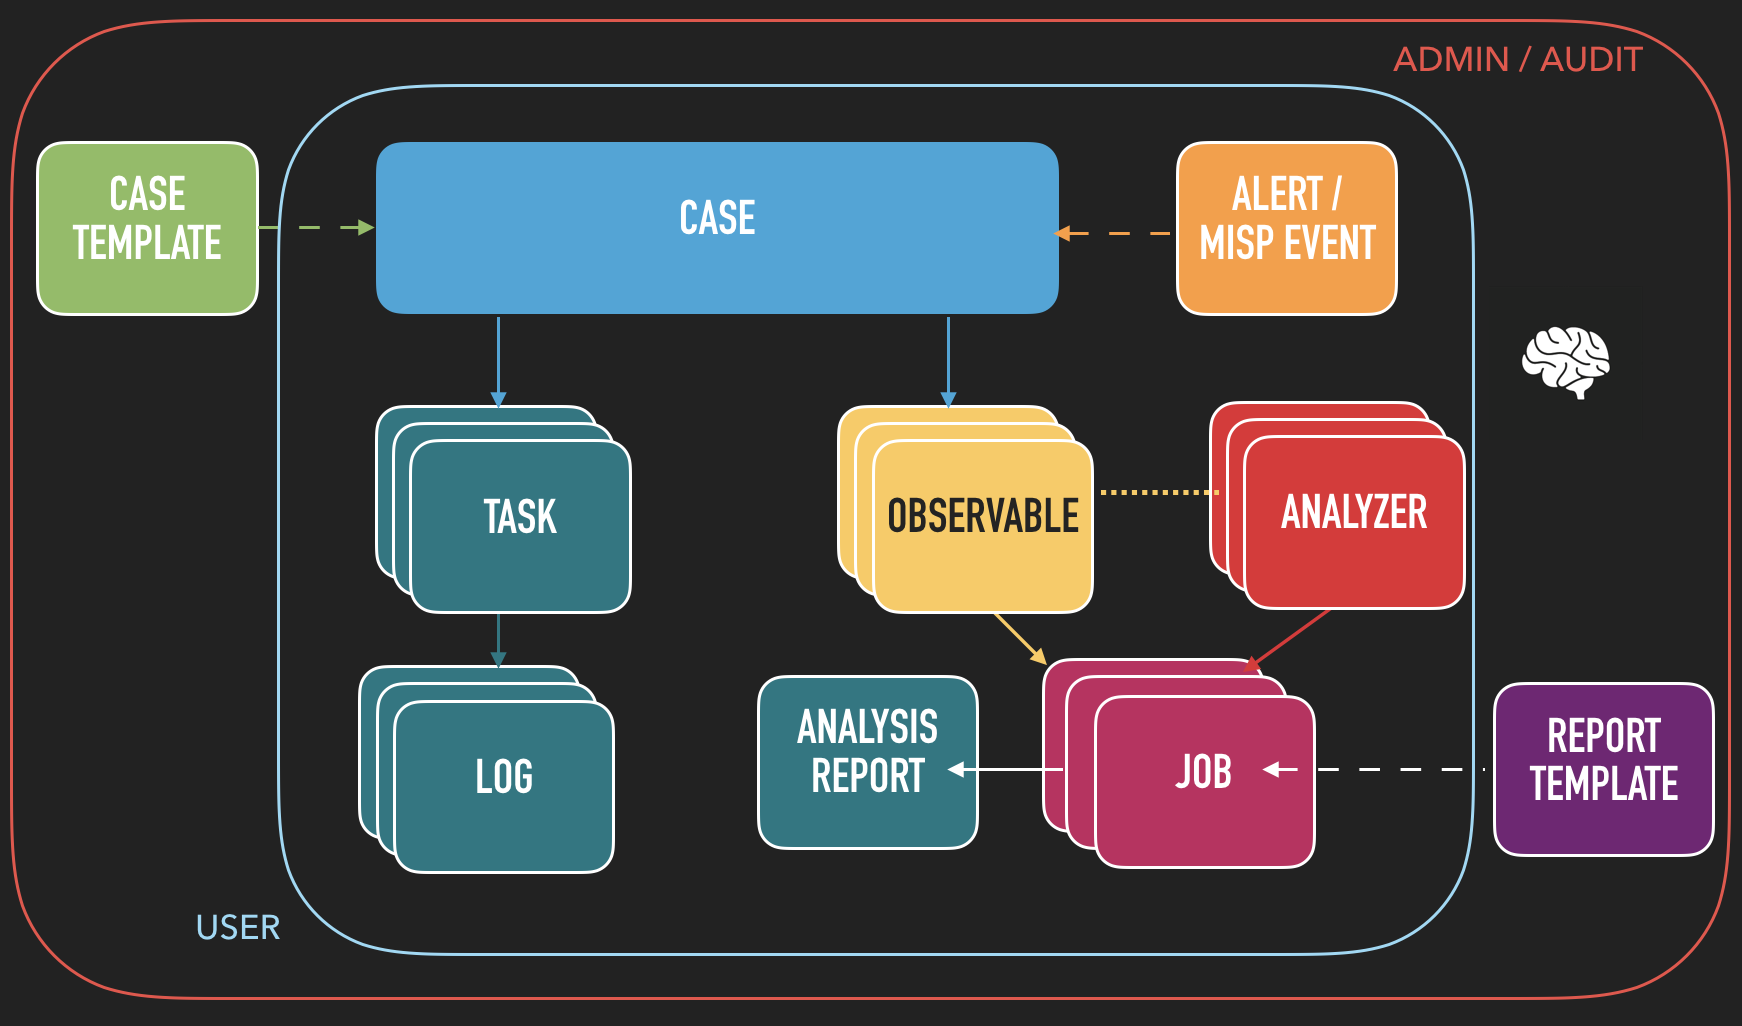
\includegraphics[width=0.79\textwidth]{thehive-workflow.png}
    \caption{Traitement d'une vulnérabilité avec TheHive}
    \label{fig:workflow}
\end{figure}

\section{Conclusion}
La mise en place de ce POC nous a permis de nous familiariser avec les indicateurs de sécurité d'une part et avec l'outil TheHive d'autre part. 
Il a le mérite de pouvoir automatiser une bonne partie du métier de l'équipe. Plus particulièrement, son niveau de scalabilité lui permettrait d'automatiser jusqu'aux envois de mail. 
\\La mise en place de ce POC n'a pas été effective. Le manque de support et la maintenance du projet ont fortement contribué à ce fait. 
\\Par ailleurs nous avons participer à la résolution de plusieurs incidents selon le process. 
Enfin, il importe de remarquer que nous avons participer à l'évolution du process actuel de l'équipe. 

\part{Intégration de la sécurité pendant la phase de développement}
\chapter{Le projet de certification continue}
\section{Introduction}
Le projet de certification continue, dans sa mise en  œuvre s'est déclinée en plusieurs étapes. Dans cette partie, nous présenterons l'existant et dégagerons les problématiques en rapport avec cet existant.

\section{Existant}
Au sein du groupe Schneider-Electric, la certification des applications se fait uniquement après la phase de développement. Durant cette phase, des tests de vulnérabilités et des tests d'intrusion sont faits sur l'application. Les rapports issus de ces tests sont renvoyés aux développeurs pour remédiation. 


\subsection{Limites du système}
Ce système présente plusieurs limites. D'abord, il laisse paraître les difficultés dans la correction du code source. En effet la remédiation des vulnérabilités pourrait demander une modification totale du code source. 
\newline
Ensuite le système demandera plusieurs ressources et allongera les temps de mise en production. Au sein du groupe, le temps de certification est de 15 jours travaillé. 
Ce temps devient vite important en considérant les tests effectués après chaque phase de remédiation.
\newline 
Enfin, ce process ne prend pas en compte la surveillance des applications. Ainsi une application déjà certifiée pourrait un jour ne plus être conforme aux normes de sécurité sans que le développeur et le propriétaire du produit ne le sachent. 


\section{Problématique}
Au regard des difficultés énoncées plus haut, il apparaît la nécessité de mettre en place un système de certification continue. Ainsi la problématique de cette partie a été de mettre en place un POC, qui permettrait d'intégrer les tests de sécurité durant la phase de développement. 

\section{Le POC}
\subsection{Objectifs}
Le POC devrait permettre de mettre en  œuvre la \ac{SDLC} de \ac{OWASP} et les principes du  \ac{DEVSECOPS}. Ces concepts permettront d'atteindre les objectifs suivants:
\begin{itemize}
    \item la réduction du temps de certification ;
    \item le développement d'applications plus sûres;
    \item la responsabilisation et la sensibilisation des développeurs sur les questions de la sécurité; 
    \item le suivi de la conformité des applications en phase d'exploitation. 
    
\end{itemize}
\subsection{Résultats attendus}
La réalisation de ce POC inclut la rédaction de plusieurs artefacts de notre part. 
En effet ce POC inclut un process, les communications, la documentation complète des outils utilisés et une implémentation technique à petite échelle.

\section{Conclusion}
La certification continue, à l'issue de ce chapitre apparaît clairement comme une nécessité au sein du groupe. 
Au vu des objectifs du POC, nous avons pu mettre la priorité sur les taches liées à la mise en place et au déploiement effectif de ce dernier.



\chapter{Gestion du projet}
\section{Introduction}
Pour mener à bien ce projet, nous avons opté pour une méthode d’organisation efficace, construite autour de la satisfaction du client et de son implication durant tout le cycle du projet. Au regard de ces exigences, notre choix s’est porté sur \ac{SCRUM}.
\newline
Il s'agit d'une méthode agile qui stipule un schéma d’organisation de développement de produits complexes. Il est défini par ses créateurs selon ses termes « un cadre de travail permettant de répondre à des problèmes complexes et changeants tout en livrant de manière productive et créative des produits de la plus grande valeur possible »

\section{les piliers de SCRUM}
\subsection{Transparence}
SCRUM met l'accent sur le fait d'avoir un langage commun entre l'équipe de développement et l’équipe de management. Ce langage commun doit permettre à tout observateur d'obtenir rapidement une bonne compréhension du projet. 

\subsection{Inspection}
À intervalles réguliers, SCRUM propose de faire le point sur les différents artéfacts produits détails, afin de détecter toute variation indésirable. Ces inspections ne doivent pas être faites trop fréquemment : cela nuirait à l'avancement du projet.


\subsection{Adaptation}
Si une dérive est constatée pendant l'inspection, le processus doit alors être adapté. SCRUM fournit des moyens rendant cette adaptation possible. Il s'agit de la réunion de planification de sprint, de la mêlée quotidienne, de la revue de sprint ainsi que de la rétrospective de sprint.

\section{Les rôles dans la gestion du projet}
SCRUM définit trois rôles : le Propriétaire du produit (Product Owner), le SCRUM Master et l’équipe de développement.

\subsection{Le propriétaire du produit}
Le propriétaire du produit (Product Owner) est le représentant des clients et des utilisateurs. Il s'agit d'« une personne et non d'un comité ». Il est seul à diriger l'activité de l'équipe de développement à qui il n'est « pas permis de suivre les instructions d'une autre personne. »
De ce fait, cet acteur se charge de différents rôles et responsabilités. Il explicite les éléments (Items) du carnet de produit (product backlog). Il définit l'ordre dans lequel les fonctionnalités seront développées. Il prend les décisions importantes concernant l'orientation du projet. Il s'assure que le carnet du produit est visible et compris de l'équipe de développement.
Dans notre cas, le propriétaire a été M. Emanuelle Beaugrand, responsable de l'équipe optimisation et la gouvernance au sein de Schneider-Electric.

\subsection{Le SCRUM master}
Le SCRUM Master est responsable de la compréhension, de l'adhésion et de la mise en œuvre de la méthode. C'est un « leader au service de l'équipe », il assiste chaque rôle de l'équipe SCRUM dans son activité. Ce n'est pas un chef de projet, ni un développeur, ni un intermédiaire de communication avec les clients. Le rôle de SCRUM Master ne peut pas être cumulé avec celui de propriétaire du produit.
Dans le cadre de notre projet, M. Jerome Bourgeon, en charge de la gestion de la performance a été le SCRUM master.

\subsection{L'équipe de développement}
L'équipe de développement a pour responsabilité de livrer à chaque fin d'itération une nouvelle version de l'application enrichie de nouvelles fonctionnalités et respectant le niveau de qualité nécessaire pour être livré. Elle est auto-organisée et choisit la façon d'accomplir son travail, sans que celle-ci soit imposée par une personne externe. Il n'y a pas non plus de notion de hiérarchie interne : toutes les décisions sont prises ensemble. Ce mode d'organisation a pour objectif d'augmenter l'efficacité de travail de l'équipe. L'équipe s'adresse directement au propriétaire du produit, et ne prend ses instructions que de lui. Son activité est issue du carnet de produit uniquement.
L'équipe de développement était composée de M. TAPSOBA Aubain 

\section{Les évènements dans le projet}
\subsection{Le sprint}
Le sprint est une période d'un mois au maximum, au bout de laquelle l'équipe délivre un incrément du produit, potentiellement livrable c’est-à-dire utilisable par le client. Une fois la durée choisie, elle reste constante pendant toute la durée du développement. Un nouveau sprint démarre dès la fin du précédent.
Chaque sprint possède un but et on lui associe une liste d'éléments du carnet du produit (fonctionnalités) à réaliser.

\subsection{La mêlée quotidienne}
La mêlée quotidienne (Daily SCRUM) est une réunion de planification « juste à temps » et permet aux développeurs de faire un point de coordination sur les tâches en cours et les difficultés rencontrées. Cette réunion dure 15 minutes au maximum. Le SCRUM Master s'assure que la réunion ait lieu à heure fixe. Le propriétaire du produit est également présent.
En ce qui concerne la mêlée quotidienne dans notre travail, nous en avons fait une adaptation suivant la disponibilité des acteurs, notamment le SCRUM master et le product owner. Ainsi, nos mêlées se faisaient chaque au besoin exprimé par l’équipe de développement.


\subsection{La réunion de planification d'itération}
Toute l'équipe SCRUM est présente à cette réunion, qui ne doit pas durer plus de 08 heures pour un sprint d'un mois. Pour un sprint plus court, la durée est réduite proportionnellement. À l'issue de cette réunion, l'équipe a décidé des éléments du carnet du produit qu'elle traitera dans le cadre de la prochaine itération, et comment elle s'organisera pour y parvenir.
La réunion de planification d'itération (Sprint Planning Meeting) se passe en deux temps. Dans la première partie, l'équipe de développement cherche à prévoir ce qui sera développé durant le prochain sprint. À l'entrée de cette phase, l'équipe doit avoir à sa disposition :
\begin{itemize}
    \item le carnet du produit priorisé ;
    \item l'incrément réalisé à la dernière itération ;
    \item la capacité de production prévue pour la prochaine itération, dont l'estimation est la prérogative de l'équipe de développement uniquement.
\end{itemize}

\begin{figure}[h!]
    \centering
    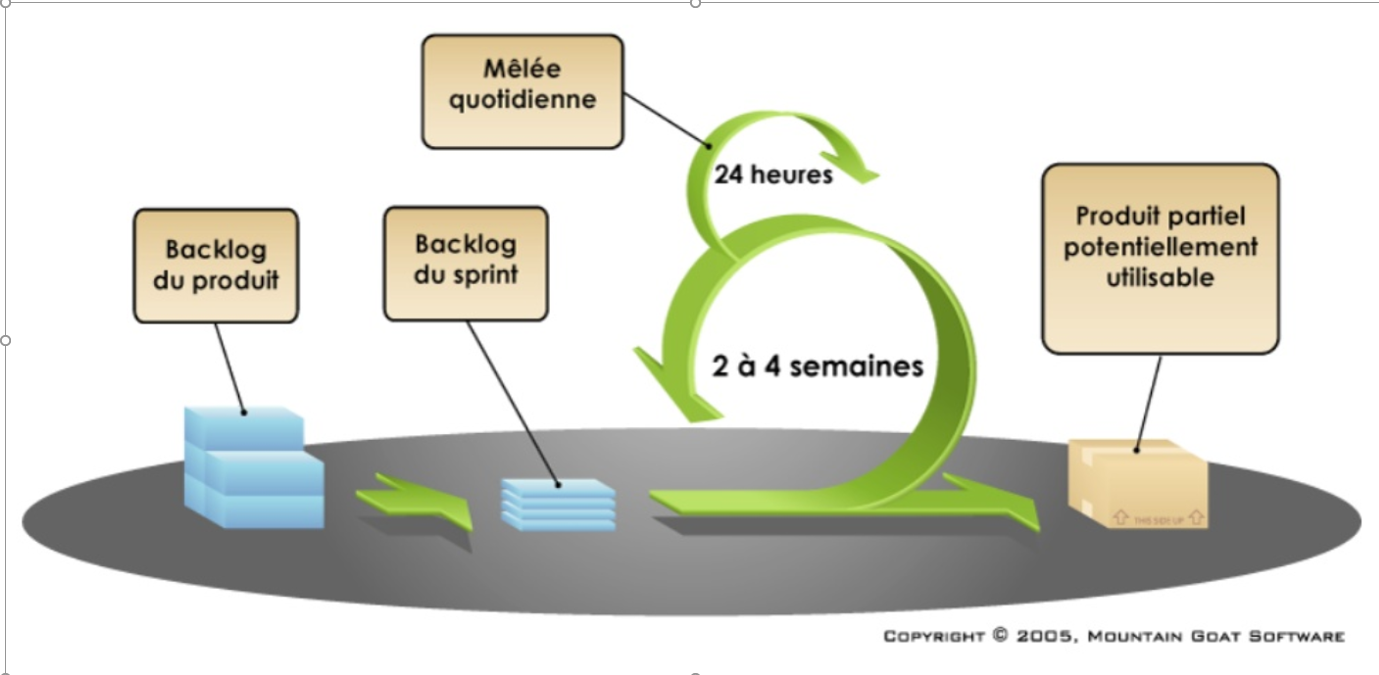
\includegraphics[width=0.9\textwidth]{scrum}
    \caption{Résumé de SCRUM}
    \label{fig:scrum}
\end{figure}

\subsection{La revue de sprint}
À la fin du sprint, l'équipe SCRUM et les parties-prenantes invitées se réunissent pour effectuer la revue de sprint, qui dure au maximum 4 heures. L'objectif de la revue de sprint est de valider l'incrément de produit qui a 
été réalisé pendant le sprint. L'équipe énonce les éléments du carnet de produit sélectionnés en début de sprint. L'équipe présente les éléments finis (complètement réalisés). Les éléments non finis (partiellement réalisés) ne sont pas présentés.
Une fois le bilan du sprint réalisé, l'équipe de développement et le propriétaire du produit mettent à jour le carnet du produit en fonction de ce qui a été réalisé (fini). Ils discutent avec les parties-prenantes de l'état courant du projet (budget, financement, conditions du marché), pour ajuster les éléments de carnet de produit et la planification selon les opportunités découvertes.

\subsection{La rétrospective du sprint}
La rétrospective du sprint est faite en interne à l'équipe SCRUM (équipe de réalisation, propriétaire du produit et SCRUM Master). Elle dure 3 heures pour un sprint d'un mois, et réduite selon la durée du sprint. Elle a pour but l'adaptation aux changements qui surviennent au cours du projet et l'amélioration continue du processus de réalisation.
L'objectif est d’inspecter l'itération précédente, afin de déterminer les éléments du processus de développement qui ont bien fonctionné et ceux qui sont à améliorer. L'équipe de développement déduit un plan d'actions d'amélioration qu'elle mettra en place lors de l'itération suivante.

\section{Les artefacts}
\subsection{Le backlog}
Le carnet de produit est « une liste ordonnée de tout ce qui pourrait être requis dans le produit et est l'unique source des besoins pour tous les changements à effectuer sur le produit ». C'est un document qui évolue constamment au cours de la vie du produit et n'est « jamais fini ».

\subsection{Le carnet de sprint} 
En début de sprint, un but est décidé. Pour atteindre cet objectif, l'équipe de développement choisit lors de la réunion de planification de sprint les éléments du carnet de produit à réaliser. Ces éléments sont alors groupés dans un carnet de sprint.

\subsection{L'incrément de produit}
L'incrément de produit est l'ensemble des éléments du carnet de produit finis pendant ce sprint, et aussi ceux finis pendant les sprints précédents. 

\subsection{Découpage du projet}
En conformité avec la méthode de gestion du projet que nous avons utilisés, la réalisation de notre POC a été découpée en backlog-sprint comme décris dans la figure [\ref{fig:backlog}] 

\begin{figure}[h!]
    \centering
    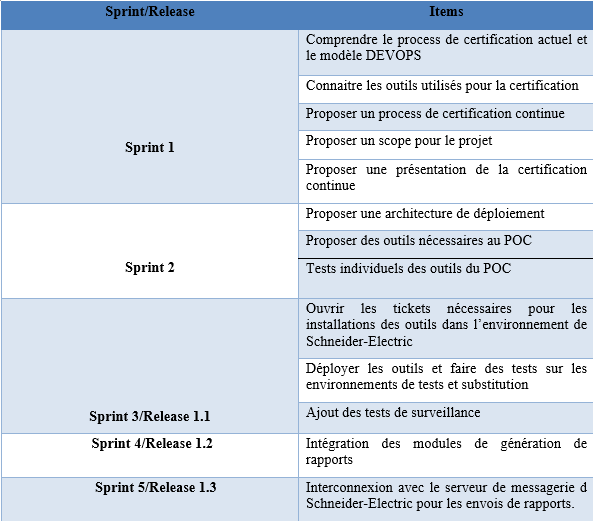
\includegraphics[width=1.0\textwidth]{backlog}
    \caption{Backlog du POC}
    \label{fig:backlog}
\end{figure}

\section*{Conclusion}
La conduite de ce façon itérative, inclusive et incrémentale nous a permis de définir et de répondre aux attentes du propriétaire du produit. SCRUM nous a garantie la flexibilité, la gestion des priorités et la conduite simplifiée du projet. 



\chapter{Mise en  œuvre}
\section{Introduction}
Dans ce chapitre nous présenterons la partie conceptuelle du POC. Il a été la base de notre travail d'implémentation. Il est le fruit de plusieurs équipes, notamment celles des développeurs, de l'équipe de certification et de celle de la sécurité. 

\section{Process}
Le process sur la figure \ref{fig:process} a été définie en concertation avec les équipes à qui le POC permettrait de  faciliter les métiers. 
Il intègre l'analyse de codes statiques et des tests de sécurité automatiques sur la couche applicative pendant la phase de développement qui seront déclenchés après chaque push de codes et des tests de conformité qui seront déclenchés après la mise en exploitation de l'application suivant une périodicité à définir par type d'application. 


\section{Périmètre du POC}
Le POC que nous avons mis en place couvre la détection de plusieurs vulnérabilités et des défauts de configuration. 
Son objectif est de couvrir les vulnérabilités web et mobiles. L'incrément que nous avons choisis d'implémenter d'abord est celui des tests de vulnérabilités des applications web. 
Ainsi, entre autres, il permettra de couvrir le top 10 de \ac{OWASP} et les vulnérabilités les plus rencontrées.  

\begin{figure}[h!]
    \centering
    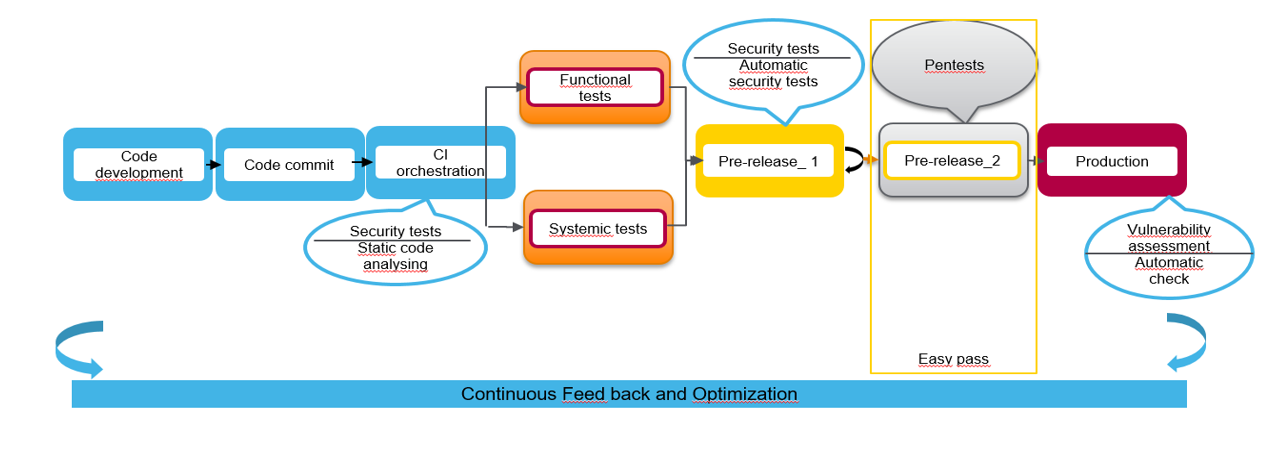
\includegraphics[width=1.17\textwidth]{process}
    \caption{Résumé du process}
    \label{fig:process}
\end{figure}
\section{Outils utilisés}
Pour la mise en place de ce process, nous avons opté pour l'utilisation des outils conventionnels et open source reconnus par les experts du monde de la sécurité informatique. 
\\La gestion du système de versionning de code a été déléguée aux outils dédiées BitBucket et Github [Cf Annexe A]. \\
L'analyse statique du code source est réservée à SonarQube[cf Annexe B]; solution open source et leader mondial dans ce domaine. 
\\Les scans de vulnérabilités en période de développement seront effectués par les outils open source OpenVas et ZAP. 
Enfin la surveillance sera uniquement effectuée par OpenVas, qui lui sera lancé sur les serveurs de tests également. 

\section{Portabilité}
La solution a pour vocation de servir plusieurs équipes utilisant souvent des technologies diverses. Face à cette contrainte, les solutions portables et faciles à dupliquer se sont imposées. C’est donc tout naturellement que nous avons choisi de déployer toutes les composantes du projet dans des conteneurs. 

\section{Considérations de sécurité}
Le système devant fournir une interface web pour l’administration, les entêtes http de sécurité ont été ajoutées afin de mitiger toute éventuelle attaque qui surviendrait au niveau de la couche applicative. Il s’agit de ces dernières : Content-Security-Policy et X-XSS-Protection.

\section{Mise à jour du POC}
La mise à jour du POC et le développement des outils à intégrer au POC incombent à l'équipe de sécurité. Elle sera en charge en plus d'organiser des communications et des formations sur les vulnérabilités les plus remontées durant les phases de tests. 


\section{Conclusion}
Dans cette partie de notre stage, nous avons pu concevoir et commencer à déployer le POC. Nous avons dans cette partie, réitérer à plusieurs reprises sur notre process. Par ailleurs, dans ce chapitre nous avons présenté les communications et les actions des équipes autour de la solution. 


\chapter*{Conclusion Générale}
Ce temps de stage au sein de l'équipe DCX-Security de la société Schneider-Electric nous a permis de travailler sur l'amélioration de la sécurité du groupe et de ses partenaires. Dans le présent document il a été question de faire le résumé de nos activité et nos réalisations durant notre stage. 


Pour ce faire nous avons divisé le document en trois parties. D'abord la première a consisté en la présentation de l'entreprise d'accueil et a permis de préciser le contexte du stage.\\ Ensuite dans la seconde, nous avons procédé à l'étude de l'existant au sein de la société et exposer nos réalisations en passant par les présentations de l'équipe d'accueil, des agences de notation et du POC de suivi des incidents. 
\\Enfin dans la troisième partie de ce document, il a été présenté nos réalisations dans l'intégration de la sécurité depuis les phases de développement. 


La sécurité informatique au sein de Schneider-Electric est à une période charnière et nous avons été ravi d'apporter notre contribution et réalisations à cette marche vers des systèmes plus sûrs. 
\\Au cours de ce stage, nous avons eu la chance d'approfondir nos connaissances sur la sécurité des applications web en particulier et sur la pratique de la sécurité en entreprise en générale. 



\appendix

\bibliographystyle{authoryear-fr}
\bibliography{references}

\clearpage

%%%%%%%%%%%%%%%%
%%% Abstract %%%
%%%%%%%%%%%%%%%%

\thispagestyle{empty}


\end{document}